\documentclass[a4paper,12pt]{report}
\usepackage[utf8x]{inputenc}
\usepackage[brazil]{babel}
\usepackage[T1]{fontenc}
\usepackage{epstopdf}
%\DeclareGraphicsRule{.tif}{png}{.png}{`convert #1 `dirname #1`/`basename #1 .tif`.png}
\usepackage{tikz}
\usepackage{indentfirst}
\hyphenation{li-vro tes-te cha-ve bi-blio-te-ca}
\hyphenation{co-men-t-rio re-fe-rn-cia}
\usetikzlibrary{positioning,shapes,shadows,arrows}
\newcommand{\HRule}{\rule{\linewidth}{0.5mm}}

\linespread{1.5}
\pagestyle{plain}


\begin{document}

%%%%%%%%%%%%%%%%%%%
% parte frontal
%%%%%%%%%%%%%%%%%%%

\begin{titlepage}

\begin{center}


\includegraphics[width=0.15\textwidth]{./logo.jpeg}\\[1cm]

\textsc{\LARGE Universidade Federal do Rio de Janeiro}\\[1.5cm]


% Title
\HRule \\[0.4cm]
{ \huge \bfseries Avaliação e Desempenho }\\[0.4cm]
{ \huge \bfseries Simulador} \\[0.4cm]
\HRule \\[1.5cm]


% Author and supervisor
\begin{minipage}{0.6\textwidth}
  \begin{flushleft} 
  \emph{Componentes:}\\
  Bruno Lima Cardoso \\
  Daniel Santos Ferreira Alves \\
  Mariam dos Passos Afonso da Conceição \\
  Peter Peret Lupo
  \end{flushleft}
\end{minipage}
\begin{minipage}{0.3\textwidth}
  \begin{flushright}
  \emph{DRE:} \\
  108055733 \\
  107362161 \\
  104034913 \\
  101137720
  \end{flushright}
\end{minipage}

\vfill

\begin{minipage}{1.0\textwidth}
  \small Bruno, Daniel e Mariam participaram ativamente, de forma remota ou presencial, de todas as etapas da elaboração do trabalho: definição do funcionamento do simulador, implementação do código, testes e produção do relatório. Peter participou das discussões, auxiliando na definição da infraestrutura do simulador e em revisões de código, fórmulas e bugs.\\
\end{minipage}

\vfill


% Bottom of the page
{\large \today}

\end{center}

\end{titlepage}

%\begin{abstract}
%\end{abstract}

\chapter*{Siglas}
\begin{list}{$\bullet$}{}
  \item[VA] - Variável Aleatória
  \item[IC] - Intervalo de Confiança
\end{list}

\chapter*{Lista de Variáveis}
\begin{list}{$\bullet$}{}
  \item[$N_{q1}$] - Número de pessoas em espera na fila 1.
  \item[$N_{q2}$] - Número de pessoas em espera na fila 2.
  \item[$N_1$] - Número de pessoas na fila 1.
  \item[$N_2$] - Número de pessoas na fila 2.
  \item[$W_1$] - Tempo de espera da fila 1.
  \item[$W_2$] - Tempo de espera da fila 2.
  \item[$X_1$] - Tempo do primeiro serviço.
  \item[$X_2$] - Tempo do segundo serviço.
  \item[$T_1$] - Tempo total de execução da fila 1.
  \item[$T_2$] - Tempo total de execução da fila 2.
  \item[$\rho$] - Utilização.
\end{list}

\tableofcontents

\listoffigures

\listoftables

%%%%%%%%%%%%%
% Introdução
%%%%%%%%%%%%%
\chapter{Introdução}

\section{Funcionamento Geral do Simulador}
O fluxo de execução do simulador é descrito, a seguir, em linhas gerais.
\begin{itemize}
  \item As estruturas internas são inicializadas e o evento inicial é gerado.
  \item Aguarda-se a execução da fase transiente.
  \item O loop principal de rodadas é iniciado. Para cada rodada:
  \begin{itemize}
    \item Se o critério de parada for satistfeito (todos os ICs são suficientemente pequenos), pare.
    \item A coleta de amostras da rodada é reiniciada.
    \item “n = eventos por rodada” eventos são retirados da fila de eventos e processados.
    \item Se não for a fase transiente, as médias da rodada são calculadas e adicionadas às listas de médias globais.
\end{itemize}
  \item Os resultados encontrados são impressos no terminal.
\end{itemize}

A execução de cada evento é descrita com detalhes na seção que trata dos tipos de eventos.

Mais detalhes sobre o funcionamento do simulador estão no \textbf{Anexo A - Workflow}.

\section{Desenvolvimento e Execução do Simulador}
A linguagem escolhida foi \textit{Java 1.6}, devido à sua portabilidade e facilidade de uso. Os gráficos foram desenhados com a ferramente \textit{GNUPlot}. Ambos estão disponíveis para Linux e Windows.

O computador usado para os testes documentados tem sistema operacional Arch Linux, processador Intel i5 e 4GB de memória RAM. Fizemos, também, um breve teste num PC com Windows XP, apenas para certificar que o simulador também era executável nesta plataforma.

Para executar o simulador em ambiente Linux, basta digitar a seguinte linha de comando: \textbf{java -jar simulador.jar}. No Windows, o mesmo comando funciona caso o JRE esteja instalado. Caso contrário, numa IDE, basta abrir o Workspace e executar o arquivo \textit{TextControl}, no pacote \textit{simulator}.

A classe \textit{TextControl} contém o cenário da simulação. Editando o método \textit{main}, podemos alterar os parâmetros da simulação (tamanho da fase transiente, fregueses por rodada, total de rodadas). Para fazermos os testes, usamos uma versão editada do código, de modo a forçar valores determinísticos.

\section{Eventos, Estruturas Internas, Métricas e Variáveis Aleatórias}
Os eventos utilizados são as chegadas nas filas, e cada fila possui um evento de chegada correspondente.

Nosso código utiliza as estruturas a seguir.
\begin{itemize}
  \item Um objeto para representa a próxima chegada na primeira fila.
  \item Uma lista para armazenar as chegadas ainda não foram servidas na segunda fila.
\end{itemize}

Não houve necessidade de usarmos uma fila de prioridades, pois os eventos já são inseridos ordenados por tempo.

Também vale destacar que temos mais de uma classe para armazenas as estatísticas coletadas:
\begin{itemize}
  \item \textit{Metrics} - coleta das estatísticas por tipo;
  \item \textit{MetricsCollection} - reúne as estatísticas de \textit{Metrics} por rodada;
  \item \textit{MetricsAgregator} - agrega os valores obtidos por cada rodada (oriundos de \textit{MetricsCollection}).
\end{itemize}

O Java possui classes prontas para fornecer números aleatórios, dentre as quais utilizamos \textit{Random} para obter números pseudo-aleatórios, entre 0 e 1, do tipo \textit{double}. Já a geração de VAs Exponenciais teve de ser implementada, papel da classe \textit{RandomExponentialVariable}. O cálculo do IC exigiu apenas um valor fixo da distribuição t-Student: o percentil \textit{$t_{0,975}$ = 1, 960}. Este valor foi armazenado na variável \textit{t}, da classe \textit{Metrics}. Outras distribuições não foram necessárias.

O método escolhido para geração das rodadas foi o \textit{Batch}, principalmente por ser necessária a realização de somente uma fase transiente, colaborando para a diminuição do tempo execução do simulador. A semente foi escolhida aleatoriamente e mantida ao longo de cada cenário.

\section{Escolha de Parâmetros}
O tamanho das rodadas e da fase transiente foi determinado empiricamente, testando-se diversos valores. Uma fase transiente inadequada, por exemplo, era indicada pela ocorrência de intervalos de confiança crescentes ao longo da simulação. Desta forma, aumentamos gradualmente o valor de seu tamanho até que os resultados fossem satisfatórios.

De forma geral, os valores foram alterados até fornecerem amostras de boa qualidade, com baixa variância e ICs que diminuíssem com mais amostras.

A tabela com os resultados dos testes controlados está na \textbf{Seção 2: Testes de Correção}, e as tabelas e gráficos dos resultados das simulações solicitadas estão na \textbf{Seção 4: Tabela com Resultados e Comentários Pertinentes}.

%%%%%%%%%%%%%
% Testes
%%%%%%%%%%%%%
\chapter{Testes de Correção}
Realizamos testes controlados para verificar a correção do simulador. Os resultado são mostrados a seguir.

\begin{table}[htbp]
  \begin{tabular}{|c|c|c|c|c|c|c|}
    \hline
    \footnotesize Classe do & \footnotesize Instante de & \footnotesize Instante de       & \footnotesize Tempo de serviço & \footnotesize Tempo      & \footnotesize Tempo   & \footnotesize Término do \\
    \footnotesize evento     & \footnotesize ocorrência  & \footnotesize processamento & \footnotesize necessário           & \footnotesize disponível & \footnotesize restante & \footnotesize tratamento \\ \hline
    1 & 0.0  & 0.0   & 1.0 & -     & -    & 1.0 \\ \hline
    2 & 1.0  & 1.0   & 1.0 & 1.0  & 0.0 & 2.0 \\ \hline
    1 & 2.0  & 2.0   & 2.0 & -      & -    & 4.0 \\ \hline
    1 & 3.0  & 4.0   & 2.0 & -      & -    & 6.0 \\ \hline
    2 & 4.0  & 6.0   & 1.0 & 2.0   & 0.0 & 7.0 \\ \hline
    2 & 6.0  & 7.0   & 2.0 & 1.0   & 0.0 & 8.0 \\ \hline
    1 & 8.0  & 8.0   & 1.0 & -      & -    & 9.0 \\ \hline
    2 & 6.0  & 9.0   & 2.0 & 11.0 & 1.0 & 10.0 \\ \hline
    2 & 9.0  & 10.0 & 1.0 & 10.0 & 0.0 & 11.0 \\ \hline
    1 & 20.0 & 11.0 & 1.0 & -     & -    & 21.0 \\ \hline
  \end{tabular}
\caption{Testes de correção}
\end{table}

A última coluna da tabela indica o momento em que terminou o tratamento do evento em questão. Os valores \textit{tempo disponível} e \textit{tempo restante} são exclusivos da classe 2. Eles indicam, respectivamente, quanto tempo um evento desta classe tinha antes de ser interrompido e quanto tempo de serviço restava, caso ele tivesse sido interrompido antes.

Enquanto variamos os valores, observamos o resultados gerados. O ajuste foi feito de acordo com o comportamento do simulador: intervalos de confiança crescentes indicavam uma da fase transiente insuficiente; resultados com variância alta sugeriam a necessidade de mais eventos ou rodadas.

Com esse teste verificamos que o contador de tempo do simulador acompanha a progressão dos eventos, que a prioridade é mantida e que as interrupções ocorrem corretamente.

%%%%%%%%%%%%%
% Fase transiente
%%%%%%%%%%%%%
\chapter{Estimativa da Fase Transiente}
Para estimar a fase transiente, analisamos o comportamento do Intervalo de Confiança. Nosso código foi estruturado de tal forma que uma escolha ruim da fase transiente não permita que ele termine sua execução, pois o crescimento do IC viola o critério de parada.

O tamanho da fase transiente é representado, na tabela com resultados, pelo \textit{número de fregueses na fase transiente}. Essa quantidade de eventos de partida desprezados varia com $\rho$.

Como citado na seção 1.2, as estatísticas foram coletas em três momentos:
\begin{itemize}
  \item ao fim do serviço de cada freguês, coletamos suas estatísticas;
  \item ao fim de cada rodada, coletamos as médias encontradas;
  \item ao fim de todas as rodadas (término da simulação), fazemos a média dos valores totais.
\end{itemize}

%\section{Método de Estimação}

%\section{Resultados do Processo}

%%%%%%%%%%%%%
% Análise
%%%%%%%%%%%%%
%tabelas com resultados e comentários pertinentes
\chapter{Tabelas com Resultados e Comentários Pertinentes}
Nesta seção mostramos tabelas com os valores dos parâmetros e das métricas obtidas em simulções com diferentes valores de $\rho$: 0.2, 0.4, 0.6, 0.8 e 0.9.

Após cada tabela existe um gráfico ilustrativo dos valores exibidos.

Os testes realizados anteriormente nos mostraram que modelamos o comportamento da fila desejada corretamente. Coletando as estatísticas, nosso intervalo de confiança tem probabilidade de 95\% de conter os valores analíticos das medidas.

\begin{table}[htbp]
  \begin{tabular}{l}
	\small Iniciando teste com ro = 0.2. \\
	\small Numero de fregueses na fase transiente: 10000 \\
	\small Numero de fregueses por rodada: 100 \\
	\small Numero de rodadas: 50 \\
	\small Total de fregueses processados: 15000 \\
	\small Resultados: \\
	\small - E[T1] = 1.1078182441545332 +- 0.0010005981628914294 \\
	\small - E[W1] = 0.11117558412968026 +- 5.000250329476253E-4 \\
	\small - E[N1] = 0.10884630051801066 +- 1.232799912896514E-4 \\
	\small - E[Nq1] = 0.010923436597187747 +- 5.167894204316871E-5 \\
	\small - E[T2] = 1.5429514728093243 +- 0.0020521837937911964 \\
	\small - E[W2] = 0.536799622380648 +- 0.001669254902107866 \\
	\small - E[N2] = 0.15157456698349814 +- 2.501820490098742E-4 \\
	\small - E[Nq2] = 0.05273371360101773 +- 1.7788037593358322E-4 \\
	\small - V(W1) = 3.254178383671827E-6 \\
	\small - V(W2) = 3.6266294359266205E-5 \\
  \end{tabular}
\caption{Resultados para $\rho$ = 0.2}
\end{table}

\begin{figure}[htbp]
   \centering
   \fbox{
	   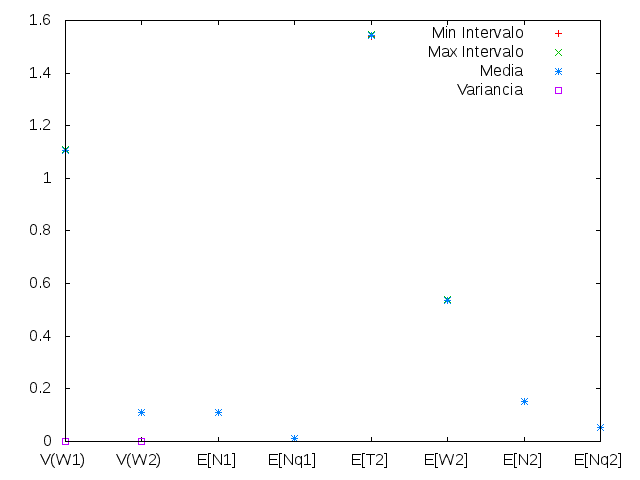
\includegraphics[width=1\textwidth]{graficos/graph-2.png}
   }\caption{Resultados para $\rho$ = 0.2}
\end{figure}

\begin{table}[htbp]
  \begin{tabular}{l}
	\small Iniciando teste com ro = 0.4. \\
	\small Numero de fregueses na fase transiente: 10000 \\
	\small Numero de fregueses por rodada: 100 \\
	\small Numero de rodadas: 100 \\
	\small Total de fregueses processados: 20000 \\
	\small Resultados: \\
	\small - E[T1] = 1.2858572348084614 +- 0.0012439714896982491 \\
	\small - E[W1] = 0.2724149470383209 +- 5.594408458229926E-4 \\
	\small - E[N1] = 0.2549654193149521 +- 1.9890460011506297E-4 \\
	\small - E[Nq1] = 0.05401530117683004 +- 9.99708270470119E-5 \\
	\small - E[T2] = 2.499839869012182 +- 0.002676192107972113 \\
	\small - E[W2] = 1.516042032628447 +- 0.002528462105154099 \\
	\small - E[N2] = 0.4955922977425739 +- 7.281645983757961E-4 \\
	\small - E[Nq2] = 0.3005556529699783 +- 6.032074885077421E-4 \\
	\small - V(W1) = 8.146971573697037E-6 \\
	\small - V(W2) = 1.6641817516660495E-4 \\
  \end{tabular}
\caption{Resultados para $\rho$ = 0.4}
\end{table}

\begin{figure}[htbp]
   \centering
   \fbox{
	   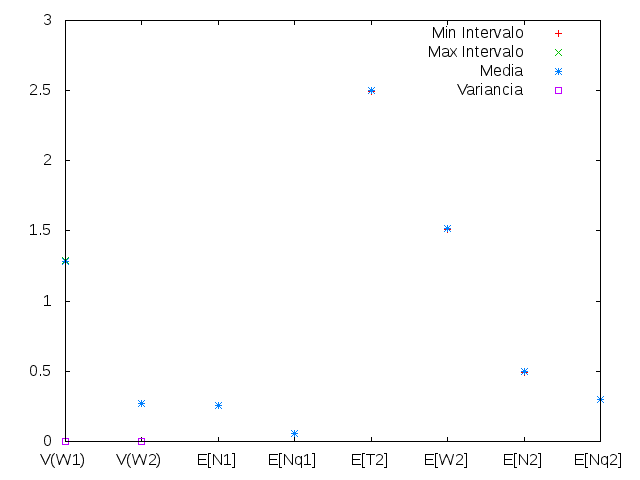
\includegraphics[width=1\textwidth]{graficos/graph-4.png}
   }\caption{Resultados para $\rho$ = 0.4}
\end{figure}

\begin{table}[htbp]
  \begin{tabular}{l}
	\small Iniciando teste com ro = 0.6. \\
	\small Numero de fregueses na fase transiente: 15000 \\
	\small Numero de fregueses por rodada: 500 \\
	\small Numero de rodadas: 100 \\
	\small Total de fregueses processados: 65000 \\
	\small Resultados: \\
	\small - E[T1] = 1.4095793607717173 +- 0.004266592226650463 \\
	\small - E[W1] = 0.41768440355047376 +- 0.0033077733769011027 \\
	\small - E[N1] = 0.4224894984492397 +- 0.0014357013072063092 \\
	\small - E[Nq1] = 0.12519730714582328 +- 0.001037275502379113 \\
	\small - E[T2] = 4.483704409912667 +- 0.034600300135734285 \\
	\small - E[W2] = 3.4836332864583968 +- 0.034142668445834405 \\
	\small - E[N2] = 1.343791637005345 +- 0.010888260052511136 \\
	\small - E[Nq2] = 1.044086381114576 +- 0.010633416618025342 \\
	\small - V(W1) = 2.848127007740453E-4 \\
	\small - V(W2) = 0.030344695142705547 \\
  \end{tabular}
\caption{Resultados para $\rho$ = 0.6}
\end{table}

\begin{figure}[htbp]
   \centering
   \fbox{
	   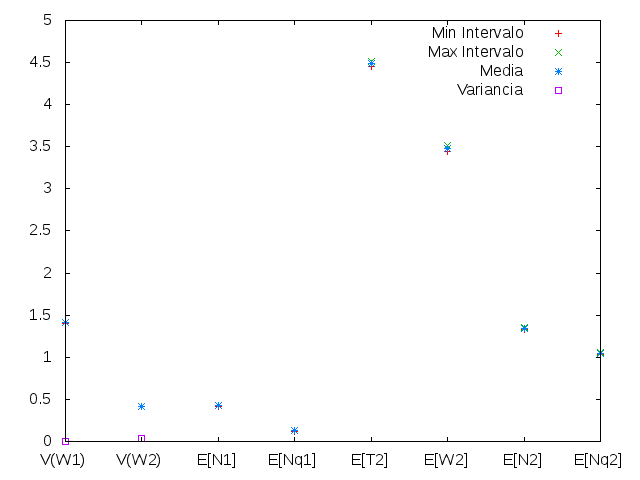
\includegraphics[width=1\textwidth]{graficos/graph-6.png}
   }\caption{Resultados para $\rho$ = 0.6}
\end{figure}

\begin{table}[htbp]
  \begin{tabular}{l}
	\small Iniciando teste com ro = 0.8. \\
	\small Numero de fregueses na fase transiente: 40000 \\
	\small Numero de fregueses por rodada: 500 \\
	\small Numero de rodadas: 100 \\
	\small Total de fregueses processados: 90000 \\
	\small Resultados: \\
	\small - E[T1] = 1.6778577086569415 +- 0.0015739632613828488 \\
	\small - E[W1] = 0.671668516897915 +- 0.0013673788815139866 \\
	\small - E[N1] = 0.6694720104354767 +- 4.429538347527855E-4 \\
	\small - E[Nq1] = 0.2679960561738116 +- 4.6465414143567144E-4 \\
	\small - E[T2] = 10.972078509242621 +- 0.033939638477058054 \\
	\small - E[W2] = 9.980079421148998 +- 0.033666456090003176 \\
	\small - E[N2] = 4.377097937355964 +- 0.01531020829120992 \\
	\small - E[Nq2] = 3.981370547971272 +- 0.015038465286372395 \\
	\small - V(W1) = 4.867047598944296E-5 \\
	\small - V(W2) = 0.029504119784988347 \\
  \end{tabular}
\caption{Resultados para $\rho$ = 0.8}
\end{table}

\begin{figure}[htbp]
   \centering
   \fbox{
	   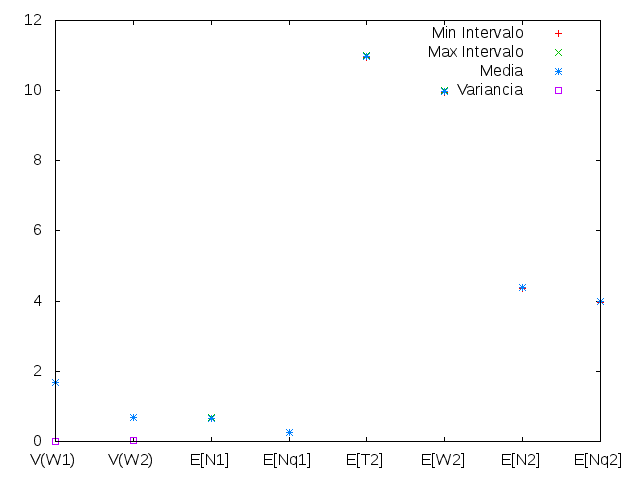
\includegraphics[width=1\textwidth]{graficos/graph-8.png}
   }\caption{Resultados para $\rho$ = 0.8}
\end{figure}

\begin{table}[htbp]
  \begin{tabular}{l}
	\small Iniciando teste com ro = 0.9. \\
	\small Numero de fregueses na fase transiente: 200000 \\
	\small Numero de fregueses por rodada: 1000 \\
	\small Numero de rodadas: 100 \\
	\small Total de fregueses processados: 300000 \\
	\small Resultados: \\
	\small - E[T1] = 1.797886987061971 +- 0.0011172524760054044 \\
	\small - E[W1] = 0.8050654947205022 +- 9.62999546674283E-4 \\
	\small - E[N1] = 0.8057137835632804 +- 6.321739914886127E-4 \\
	\small - E[Nq1] = 0.36078685406245037 +- 4.913982377772008E-4 \\
	\small - E[T2] = 24.72219616289994 +- 0.07293770230754473 \\
	\small - E[W2] = 23.72095202157548 +- 0.07288675037239704 \\
	\small - E[N2] = 11.07786120869003 +- 0.03454485349707596 \\
	\small - E[Nq2] = 10.629215660822135 +- 0.034447382153444325 \\
	\small - V(W1) = 2.4140153240703732E-5 \\
	\small - V(W2) = 0.13828817107059876 \\
  \end{tabular}
\caption{Resultados para $\rho$ = 0.9}
\end{table}

\begin{figure}[htbp]
   \centering
   \fbox{
	   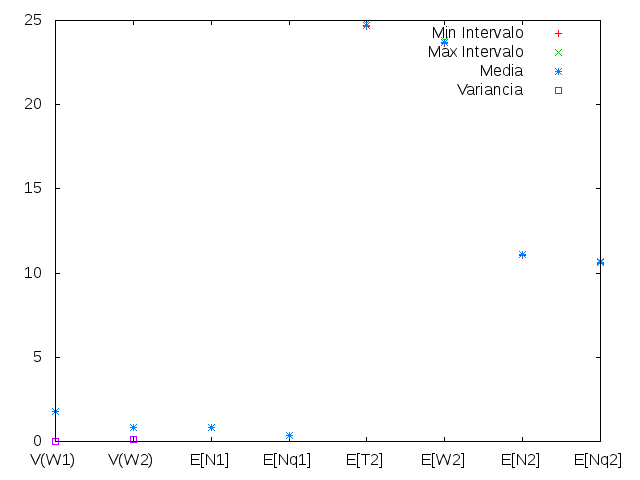
\includegraphics[width=1\textwidth]{graficos/graph-9.png}
   }\caption{Resultados para $\rho$ = 0.9}
\end{figure}

%%%%%%%%%%%%%
% Otimização
%%%%%%%%%%%%%
\chapter{Otimização}
Através dos testes empíricos cremos ter conseguido atingir boas combinações para os parâmetros do simulador. Como citado anteriormente, nosso objetivo foi obter amostras de boa qualidade, com baixa variância e ICs que diminuíssem conforme aumentamos a quantidade de amostras.

%\section{Apresentação do Método}

%\section{Análise Gráfica de Resultados}

%%%%%%%%%%%%%
% Conclusão
%%%%%%%%%%%%%
\chapter{Conclusão}
Definir a infraestrutura do código do simulador foi uma tarefa que exigiu dos participantes do grupo conhecimentos não só da linguagem escolhida, mas, principalmente, da Teoria  de Filas. Ambos foram fundamentais no decorrer do desenvolvimento deste trabalho. Ao mesmo tempo, pudemos aprimorar nossos conhecimentos teóricos.

A maior dificuldade encontrada foi a realização dos testes, devido à necessidade de analisar cuidadosamente as medidas geradas e, simultaneamente, modificar o código para ajustar sua correção. Além disso, todos os cálculos foram verificados para evitar erros.

Alguns trabalhos futuros interessantes sobre nosso código seriam a integração de uma interface gráfica e a possibilidade de gerar os gráficos internamente.

%%%%%%%%%%%%%%%%%%%
% parte final
%%%%%%%%%%%%%%%%%%%
\appendix
\chapter{Workflow}

\newpage

\appendix
\chapter{O Programa}

\end{document}          
